\documentclass[11pt,a4paper]{article}

% --- Page Margins ---
\usepackage[a4paper, top=2.4cm, bottom=2.4cm, left=2.2cm, right=2.2cm]{geometry}

% --- Font Configuration: Times New Roman ---
\usepackage{iftex}
\ifTUTeX
    \usepackage{fontspec}
    \IfFontExistsTF{Times New Roman}{
        \setmainfont{Times New Roman}
    }{
        \setmainfont{TeX Gyre Termes}
    }
\else
    \usepackage[utf8]{inputenc}
    \usepackage[T1]{fontenc}
    \usepackage{mathptmx}
\fi

% --- Line Spacing: 20 pt (11pt default baselineskip is 13.6pt; 13.6 * 1.47 = 20pt) ---
\linespread{1.47}

% --- Math, Typography, Graphics, and Layout Packages ---
\usepackage{amsmath,amssymb,amsthm}
\usepackage{parskip}
\usepackage{enumitem}
\usepackage{xcolor}
\usepackage{float}
\usepackage{tikz}
\usetikzlibrary{arrows.meta, decorations.markings}

% --- List Spacing Refinement ---
\setlist[itemize]{itemsep=2pt, topsep=3pt, parsep=2pt, leftmargin=1.6em}
\setlist[enumerate]{itemsep=2pt, topsep=3pt, parsep=2pt, leftmargin=1.8em}

% --- Custom Theorem & Definition Styles (Header on its own line) ---
\newtheoremstyle{definitionbreak}
  {10pt}        % Space above
  {10pt}        % Space below
  {\normalfont} % Body font
  {0pt}         % Indent amount
  {\bfseries\color{blue!60!black}} % Theorem head font
  {.}           % Punctuation after theorem head
  {\newline}    % Space after theorem head (starts body on a new line)
  {\thmname{#1}\thmnumber{ #2}\thmnote{ \textnormal{\textbf{(#3)}}}}

\newtheoremstyle{examplebreak}
  {10pt}        % Space above
  {10pt}        % Space below
  {\normalfont} % Body font
  {0pt}         % Indent amount
  {\bfseries\color{teal!65!black}} % Theorem head font
  {.}           % Punctuation after theorem head
  {\newline}    % Space after theorem head (starts body on a new line)
  {\thmname{#1}\thmnumber{ #2}\thmnote{ \textnormal{\textbf{(#3)}}}}

\theoremstyle{definitionbreak}
\newtheorem{definition}{Definition}

\theoremstyle{examplebreak}
\newtheorem{example}{Example}

\theoremstyle{plain}
\newtheorem{theorem}{Theorem}
\newtheorem{proposition}{Proposition}
\newtheorem{lemma}{Lemma}

% --- Hyperref (Must be loaded last) ---
\usepackage[colorlinks=true, linkcolor=blue!60!black, urlcolor=blue!60!black]{hyperref}

\begin{document}

% ==================================================
% Title and Instructor Information
% ==================================================
\begin{center}
    {\LARGE \textbf{Mathematics Method for Physics -- Lecture 3}} \\[0.4em]
    {\large Functions of a Complex Variable and Elementary Complex Functions}
\end{center}

\vspace{-0.4em}
\noindent\rule{\textwidth}{0.6pt}
\vspace{0.1em}

\begin{center}
    Instructor: Zhaolong Han, SOCE, Shanghai Jiao Tong University \quad|\quad Email: \texttt{han.arkey@sjtu.edu.cn}
\end{center}

\vspace{0.1em}
\noindent\rule{\textwidth}{0.6pt}

\vspace{0.5em}
\noindent \textit{Overview: These lecture notes cover functions of a complex variable as geometric mappings and the five classes of elementary complex functions.}

\vspace{0.8em}

% ==================================================
% Section 1: Functions of a Complex Variable
% ==================================================
\section{Functions of a Complex Variable}

\subsection{Concept of Complex Functions and Geometric Mappings}

\begin{definition}[Complex Function]
Let $D$ be a point set in the complex plane $\mathbb{C}$. If for every complex number $z \in D$, there corresponds one or more complex numbers $w$ according to a rule $f$, then $w$ is called a \textbf{function of a complex variable} defined on $D$, denoted by
\[
    w = f(z), \quad z \in D.
\]
Here $D$ is the \textbf{domain of definition}, and $G = \{ w = f(z) \mid z \in D \}$ is the \textbf{range} (image set).
\end{definition}

\textbf{Structural and Geometric Properties}:
\begin{itemize}
    \item \textbf{Single-valued vs. Multi-valued Functions}: If each $z \in D$ corresponds to a unique value $w$, $f(z)$ is called \emph{single-valued} (e.g., $w = z^2$, $w = |z|$); if $z$ corresponds to two or more values, $f(z)$ is called \emph{multi-valued} (e.g., $w = \operatorname{Arg} z$, $w = \sqrt[n]{z}$).
    \item \textbf{Real and Imaginary Decomposition}: Writing $z = x + iy$ and $w = u + iv$, a complex function is equivalent to a pair of real-valued functions of two real variables:
    \[
        w = f(z) = u(x, y) + i v(x, y).
    \]
    \item \textbf{Inverse Function}: If for each $w \in G$ there exist one or more points $z \in D$ satisfying $w = f(z)$, this correspondence defines the inverse function $z = g(w) = f^{-1}(w)$.
    \item \textbf{Geometric Interpretation as a Mapping}: Unlike a real function $y = f(x)$ which can be visualized as a curve in $\mathbb{R}^2$, a complex function $w = f(z)$ involves four real dimensions $(x, y, u, v)$ and cannot be plotted as a graph in low dimensions. Instead, we interpret $w = f(z)$ as a \textbf{mapping} (or transformation) from a set $D$ in the $z$-plane to its image $G$ in the $w$-plane (which may be injective/one-to-one, surjective/onto, or bijective).
\end{itemize}

\begin{example}[Mapping Properties of $w = z^2$]
Let $z = x + iy = r e^{i\theta}$ and $w = u + iv = \rho e^{i\varphi}$. For $w = z^2$, we have
\[
    u = x^2 - y^2, \quad v = 2xy \qquad \text{and} \qquad \rho = r^2, \quad \varphi = 2\theta + 2k\pi.
\]
\begin{enumerate}
    \item \textbf{Image of the Real Axis}: On the real axis $y = 0$, we obtain $u = x^2 \ge 0$ and $v = 0$. Thus, $w = z^2$ maps the real axis of the $z$-plane onto the non-negative real axis $[0, +\infty)$ of the $w$-plane, covering $(0, +\infty)$ twice—once for $x > 0$ and once for $x < 0$ (see Figure 1). Similarly, the imaginary axis $x = 0$ maps onto the non-positive real axis $(-\infty, 0]$.
    \item \textbf{Image of Angular Sectors}: The angular sector $0 < \arg z < \alpha$ ($0 < \alpha \le \pi$) is mapped onto the sector $0 < \arg w < 2\alpha$ (see Figure 2). In particular, the first quadrant $0 < \arg z < \frac{\pi}{2}$ is mapped one-to-one onto the upper half-plane $0 < \arg w < \pi$.
\end{enumerate}
\end{example}

% --- Figure 1: Mapping of the Real Axis ---
\begin{figure}[H]
\centering
\begingroup
\linespread{1.0}\selectfont
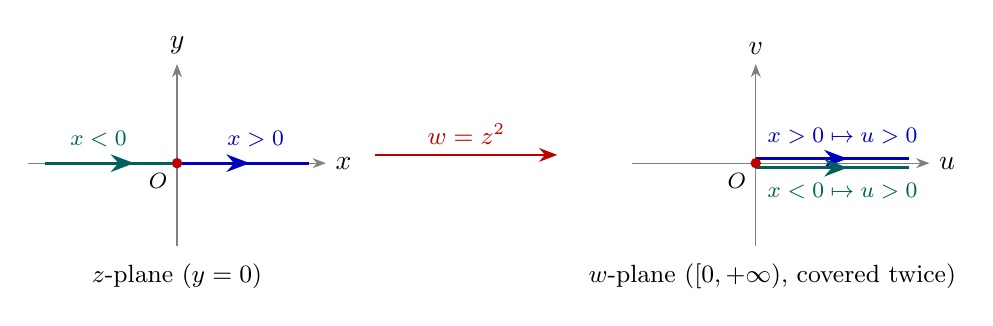
\begin{tikzpicture}[scale=1.05, >=Stealth]
    % Left: z-plane
    \begin{scope}[shift={(-3.5, 0)}]
        \draw[->, gray] (-1.8, 0) -- (1.8, 0) node[right, black] {$x$};
        \draw[->, gray] (0, -1.0) -- (0, 1.2) node[above, black] {$y$};
        % Negative real axis (x < 0)
        \draw[very thick, teal!75!black, postaction={decorate}, decoration={markings, mark=at position 0.5 with {\arrow{<}}}] (0,0) -- (-1.6,0);
        \node[teal!75!black, above, font=\footnotesize] at (-0.95, 0.08) {$x < 0$};
        % Positive real axis (x > 0)
        \draw[very thick, blue!75!black, postaction={decorate}, decoration={markings, mark=at position 0.55 with {\arrow{>}}}] (0,0) -- (1.6,0);
        \node[blue!75!black, above, font=\footnotesize] at (0.95, 0.08) {$x > 0$};
        % Origin
        \fill[red!75!black] (0,0) circle (1.8pt) node[below left, black, font=\footnotesize] {$O$};
        \node[below, font=\small] at (0, -1.1) {$z$-plane ($y = 0$)};
    \end{scope}

    % Mapping Arrow
    \draw[->, thick, red!75!black] (-1.1, 0.1) -- (1.1, 0.1) node[midway, above, font=\small] {$w = z^2$};

    % Right: w-plane
    \begin{scope}[shift={(3.5, 0)}]
        \draw[->, gray] (-1.5, 0) -- (2.1, 0) node[right, black] {$u$};
        \draw[->, gray] (0, -1.0) -- (0, 1.2) node[above, black] {$v$};
        % Double cover of [0, +infty)
        \draw[very thick, blue!75!black, postaction={decorate}, decoration={markings, mark=at position 0.6 with {\arrow{>}}}] (0, 0.055) -- (1.85, 0.055);
        \draw[very thick, teal!75!black, postaction={decorate}, decoration={markings, mark=at position 0.6 with {\arrow{>}}}] (0, -0.055) -- (1.85, -0.055);
        \node[blue!75!black, above, font=\footnotesize] at (1.05, 0.12) {$x > 0 \mapsto u > 0$};
        \node[teal!75!black, below, font=\footnotesize] at (1.05, -0.12) {$x < 0 \mapsto u > 0$};
        % Origin
        \fill[red!75!black] (0,0) circle (1.8pt) node[below left, black, font=\footnotesize] {$O$};
        \node[below, font=\small] at (0.2, -1.1) {$w$-plane ($[0, +\infty)$, covered twice)};
    \end{scope}
\end{tikzpicture}
\caption{Geometric action of $w = z^2$ on the real axis ($y = 0$): the positive ($x > 0$) and negative ($x < 0$) real axes fold onto $[0, +\infty)$ twice.}
\endgroup
\end{figure}

% --- Figure 2: Mapping of Angular Sector ---
\begin{figure}[H]
\centering
\begingroup
\linespread{1.0}\selectfont
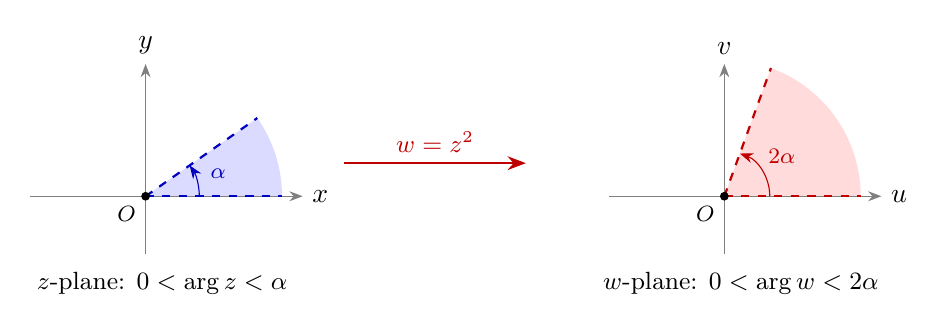
\begin{tikzpicture}[scale=1.05, >=Stealth]
    % Left: z-plane
    \begin{scope}[shift={(-3.5, 0)}]
        % Shaded sector 0 < arg z < 35 deg
        \fill[blue!14!white] (0,0) -- (1.65,0) arc (0:35:1.65cm) -- cycle;
        \draw[->, gray] (-1.4, 0) -- (1.9, 0) node[right, black] {$x$};
        \draw[->, gray] (0, -0.7) -- (0, 1.6) node[above, black] {$y$};
        % Boundary rays (dashed for open sector)
        \draw[thick, dashed, blue!75!black] (0,0) -- (1.65, 0);
        \draw[thick, dashed, blue!75!black] (0,0) -- (35:1.65cm);
        % Angle arc
        \draw[->, blue!75!black] (0.65,0) arc (0:35:0.65cm);
        \node[blue!75!black, font=\footnotesize] at (17.5:0.92cm) {$\alpha$};
        \fill[black] (0,0) circle (1.5pt) node[below left, font=\footnotesize] {$O$};
        \node[below, font=\small] at (0.2, -0.8) {$z$-plane: $0 < \arg z < \alpha$};
    \end{scope}

    % Mapping Arrow
    \draw[->, thick, red!75!black] (-1.1, 0.4) -- (1.1, 0.4) node[midway, above, font=\small] {$w = z^2$};

    % Right: w-plane
    \begin{scope}[shift={(3.5, 0)}]
        % Shaded sector 0 < arg w < 70 deg
        \fill[red!14!white] (0,0) -- (1.65,0) arc (0:70:1.65cm) -- cycle;
        \draw[->, gray] (-1.4, 0) -- (1.9, 0) node[right, black] {$u$};
        \draw[->, gray] (0, -0.7) -- (0, 1.6) node[above, black] {$v$};
        % Boundary rays (dashed for open sector)
        \draw[thick, dashed, red!75!black] (0,0) -- (1.65, 0);
        \draw[thick, dashed, red!75!black] (0,0) -- (70:1.65cm);
        % Angle arc
        \draw[->, red!75!black] (0.55,0) arc (0:70:0.55cm);
        \node[red!75!black, font=\footnotesize] at (35:0.85cm) {$2\alpha$};
        \fill[black] (0,0) circle (1.5pt) node[below left, font=\footnotesize] {$O$};
        \node[below, font=\small] at (0.2, -0.8) {$w$-plane: $0 < \arg w < 2\alpha$};
    \end{scope}
\end{tikzpicture}
\caption{Geometric action of $w = z^2$ on an angular sector: an open sector $0 < \arg z < \alpha$ maps onto $0 < \arg w < 2\alpha$, doubling the opening angle.}
\endgroup
\end{figure}

\subsection{Elementary Complex Functions}

Elementary functions of a complex variable are grouped into \textbf{five major categories}, extending real elementary functions to $\mathbb{C}$ while preserving algebraic identities.

\subsubsection{1. Exponential Function}

\begin{definition}[Complex Exponential Function]
For any complex number $z = x + iy$, the exponential function is defined by
\[
    w = e^z = \exp(z) = e^{x + iy} = e^x (\cos y + i \sin y).
\]
\end{definition}

\textbf{Properties of $e^z$}:
\begin{enumerate}
    \item \textbf{Modulus and Argument}: $|e^z| = e^x > 0$ (hence $e^z \neq 0$ for all $z \in \mathbb{C}$), and $\operatorname{Arg}(e^z) = y + 2k\pi$ ($k \in \mathbb{Z}$).
    \item \textbf{Real, Imaginary, and Conjugate Parts}:
    \[
        \operatorname{Re}(e^z) = e^x \cos y, \quad \operatorname{Im}(e^z) = e^x \sin y, \quad \overline{e^z} = e^x(\cos y - i\sin y) = e^{\overline{z}}.
    \]
    \item \textbf{Addition Property}: For all $z_1, z_2 \in \mathbb{C}$, $e^{z_1} \cdot e^{z_2} = e^{z_1 + z_2}$. (Note: $(e^{z_1})^{z_2} = e^{z_1 z_2}$ does not hold in general due to multi-valuedness.)
    \item \textbf{Periodicity}: Since $e^{2k\pi i} = 1$, $e^z$ is periodic with fundamental period $T = 2\pi i$:
    \[
        e^{z + 2k\pi i} = e^z \quad (k = 0, \pm 1, \pm 2, \dots).
    \]
    \item \textbf{Analyticity and Behavior at $\infty$}: $e^z$ is analytic on the entire complex plane $\mathbb{C}$ with $(e^z)' = e^z$, and $\lim_{z \to \infty} e^z$ does not exist.
\end{enumerate}

\subsubsection{2. Logarithmic Function}

\begin{definition}[Complex Logarithmic Function]
For $z \neq 0, \infty$, any complex number $w$ satisfying $e^w = z$ is called the logarithm of $z$, denoted by $w = \operatorname{Ln} z$. Writing $z = r e^{i\theta}$ and $w = u + iv$, we obtain
\[
    w = \operatorname{Ln} z = \ln|z| + i\operatorname{Arg} z = \ln|z| + i(\arg z + 2k\pi) \quad (k = 0, \pm 1, \pm 2, \dots).
\]
\end{definition}

\textbf{Properties of $\operatorname{Ln} z$}:
\begin{enumerate}
    \item \textbf{Principal Value and Branches}: Fixing $k$ yields a single-valued branch. For $k = 0$, we obtain the \textbf{principal value}:
    \[
        \ln z = \ln|z| + i\arg z \quad (-\pi < \arg z \le \pi),
    \]
    where $\operatorname{Re}(\ln z) = \ln|z|$ and $\operatorname{Im}(\ln z) = \arg z$. Thus $\operatorname{Ln} z = \ln z + 2k\pi i$.
    \item \textbf{Example}: $\operatorname{Ln}(-1) = \ln|-1| + i(\pi + 2k\pi) = (2k + 1)\pi i$, with principal value $\ln(-1) = \pi i$.
    \item \textbf{Algebraic Identities}: For $z_1, z_2 \neq 0$, as equalities between sets of values:
    \[
        \operatorname{Ln}(z_1 z_2) = \operatorname{Ln} z_1 + \operatorname{Ln} z_2, \qquad \operatorname{Ln}\left(\frac{z_1}{z_2}\right) = \operatorname{Ln} z_1 - \operatorname{Ln} z_2.
    \]
    \emph{Warning}: For principal values, $\ln(z_1 z_2) = \ln z_1 + \ln z_2$ \textbf{does not always hold} (e.g., when $\arg z_1 + \arg z_2 \notin (-\pi, \pi]$).
    \item \textbf{Analyticity}: Every branch of $\operatorname{Ln} z$ is analytic on the slit plane $\mathbb{C} \setminus (-\infty, 0]$ with derivative $(\operatorname{Ln} z)' = \frac{1}{z}$.
\end{enumerate}

\subsubsection{3. Power Function and General Exponential Function}

\begin{definition}[Complex Power Function]
For any complex exponent $a \in \mathbb{C}$ and $z \neq 0$, the power function is defined via the exponential and logarithmic functions as
\[
    w = z^a = e^{a \operatorname{Ln} z} = e^{a(\ln|z| + i\arg z + 2k\pi i)} = e^{a \ln z} \cdot e^{2k\pi a i} \quad (k = 0, \pm 1, \pm 2, \dots).
\]
Similarly, for $a \neq 0$, the general exponential function is defined as $w = a^z = e^{z \operatorname{Ln} a}$ (which is multi-valued when $a \neq e$).
\end{definition}

\textbf{Classification by Exponent $a$}:
\begin{itemize}
    \item $a = n \in \mathbb{Z}^+$: $w = z^n = r^n e^{in\theta}$ is single-valued and entire on $\mathbb{C}$.
    \item $a = -n$ ($n \in \mathbb{Z}^+$): $w = z^{-n} = \frac{1}{z^n}$ is single-valued and analytic on $\mathbb{C} \setminus \{0\}$.
    \item $a = \frac{1}{n}$ ($n \in \mathbb{Z}^+$): $w = z^{1/n} = \sqrt[n]{z} = \sqrt[n]{r} e^{i\frac{\theta + 2k\pi}{n}}$ ($k = 0, 1, \dots, n-1$) is $n$-valued.
    \item $a = \frac{m}{n}$ (reduced fraction, $n > 1$): $w = z^{m/n}$ is $n$-valued.
    \item Other $a$ (irrational or non-real complex): $w = z^a$ is infinitely many-valued.
\end{itemize}

\begin{example}[Evaluation of $i^i$]
Compute all values of the multi-valued power $i^i$:
\[
    i^i = e^{i \operatorname{Ln} i} = e^{i\left[\ln|i| + i\left(\frac{\pi}{2} + 2k\pi\right)\right]} = e^{-\frac{\pi}{2} - 2k\pi} \quad (k = 0, \pm 1, \pm 2, \dots).
\]
Notice that all infinitely many values of $i^i$ are positive real numbers!
\end{example}

\subsubsection{4. Trigonometric and Hyperbolic Functions}

\begin{definition}[Complex Trigonometric Functions]
Extending Euler's formula $e^{ix} = \cos x + i\sin x$ ($x \in \mathbb{R}$) to $z \in \mathbb{C}$, the sine and cosine functions are defined as
\[
    \sin z = \frac{e^{iz} - e^{-iz}}{2i}, \qquad \cos z = \frac{e^{iz} + e^{-iz}}{2}.
\]
The remaining trigonometric functions are defined by
\[
    \tan z = \frac{\sin z}{\cos z}, \quad \cot z = \frac{\cos z}{\sin z}, \quad \sec z = \frac{1}{\cos z}, \quad \csc z = \frac{1}{\sin z}.
\]
\end{definition}

\textbf{Properties of Complex Trigonometric Functions}:
\begin{enumerate}
    \item \textbf{Euler's Formula}: $e^{iz} = \cos z + i\sin z$ holds for all $z \in \mathbb{C}$.
    \item \textbf{Periodicity and Parity}: $\sin z$ and $\cos z$ are periodic with period $2\pi$; $\sin(-z) = -\sin z$ (odd) and $\cos(-z) = \cos z$ (even).
    \item \textbf{Analyticity and Identities}: $\sin z$ and $\cos z$ are entire functions with $(\sin z)' = \cos z$ and $(\cos z)' = -\sin z$. Standard real identities ($\sin^2 z + \cos^2 z = 1$, sum/difference formulas) remain valid.
    \item \textbf{Zeros}: All zeros lie on the real axis: $\sin z = 0 \iff z = k\pi$, and $\cos z = 0 \iff z = k\pi + \frac{\pi}{2}$ ($k \in \mathbb{Z}$).
    \item \textbf{Unboundedness}: Unlike real sine and cosine, $|\sin z|$ and $|\cos z|$ are \textbf{unbounded} on $\mathbb{C}$ (e.g., $|\cos(iy)| = \cosh y \to +\infty$ as $|y| \to \infty$).
\end{enumerate}

\begin{definition}[Complex Hyperbolic Functions]
The hyperbolic sine, cosine, and tangent functions are defined for $z \in \mathbb{C}$ by
\[
    \sinh z = \frac{e^z - e^{-z}}{2}, \qquad \cosh z = \frac{e^z + e^{-z}}{2}, \qquad \tanh z = \frac{\sinh z}{\cosh z}.
\]
\end{definition}

They satisfy $\sinh z = -i\sin(iz)$, $\cosh z = \cos(iz)$, $\cosh^2 z - \sinh^2 z = 1$, $(\sinh z)' = \cosh z$, and $(\cosh z)' = \sinh z$, with fundamental period $2\pi i$.

\subsubsection{5. Inverse Trigonometric and Inverse Hyperbolic Functions}

Defined as the inverse mappings of the trigonometric and hyperbolic functions, these functions are all infinitely many-valued:
\begin{align*}
    \operatorname{Arcsin} z &= -i\operatorname{Ln}\left(iz \pm \sqrt{1 - z^2}\right), & \operatorname{Arccos} z &= -i\operatorname{Ln}\left(z \pm \sqrt{z^2 - 1}\right), \\[6pt]
    \operatorname{Arctan} z &= -\frac{i}{2}\operatorname{Ln}\frac{1 + iz}{1 - iz} \quad (z \neq \pm i), & \operatorname{Arccot} z &= \frac{i}{2}\operatorname{Ln}\frac{z - i}{z + i} \quad (z \neq \pm i), \\[6pt]
    \operatorname{Arcsinh} z &= \operatorname{Ln}\left(z \pm \sqrt{z^2 + 1}\right), & \operatorname{Arccosh} z &= \operatorname{Ln}\left(z \pm \sqrt{z^2 - 1}\right).
\end{align*}

% ==================================================
% Assigned Homework Reference
% ==================================================
\vspace{0.8em}
\noindent\rule{\textwidth}{0.5pt}
\section*{Assigned Homework Reference}
\begin{itemize}
    \item \textbf{Textbook P.20 (Exercise 1)}: Set A: Problems 8 (even), 9, 12; \quad Set B: Problems 5, 6.
    \item \textbf{Textbook P.55 (Exercise 2)}: Set A: Problem 13 (even).
\end{itemize}

\end{document}